% =====================================================================
%  Final-project poster: 3-column, landscape
%  Page: 48 in x 32.2 in  -> aspect 1.4907 (identical to the 1024x687
%  sample poster).  Compile with pdfLaTeX (Overleaf default).
%
%  HOW TO USE
%   1. Upload this file and the figures/ folder to Overleaf.
%   2. Any missing image is drawn as a dashed placeholder box, so the
%      poster always compiles.
%   3. The data figures are redrawn with  python3 scripts/make_figures.py
%
%  PRINT-FRIENDLY: no black or dark fills.  Black is used for text only;
%  highlights use RIT orange and the teal accent (ritteal).
% =====================================================================
\documentclass{article}

% ---------------- page geometry (same aspect ratio as sample) --------
\usepackage[paperwidth=48in, paperheight=32.2in,
            left=0.75in, right=0.75in,
            top=4.20in, bottom=3.70in]{geometry}

% ---------------- fonts ---------------------------------------------
\usepackage[T1]{fontenc}
\usepackage{lmodern}                 % scalable math fonts
\usepackage{tgheros}                 % Helvetica-style text font
\renewcommand*\familydefault{\sfdefault}
\usepackage{anyfontsize}
\usepackage{microtype}
\usepackage{fontawesome5}

% ---------------- graphics / layout ---------------------------------
\usepackage{etoolbox}
\usepackage{xcolor}
\usepackage{graphicx}
\usepackage{tikz}
\usetikzlibrary{arrows.meta,positioning,calc,shapes.misc}
\usepackage{eso-pic}
\usepackage{enumitem}
\usepackage[most]{tcolorbox}

% =====================================================================
%  POSTER IDENTITY
% =====================================================================
\newcommand{\PosterTitle}{Tracking the Coqu\'i Frog: Autonomous Navigation in Unstructured Environments}
\newcommand{\PosterTagline}{Hear it. Find it. Photograph it.\quad No GPS, no map, no AI.}
\newcommand{\AuthorName}{Manvith Reddy Dayam}
\newcommand{\AuthorEmail}{md1649@g.rit.edu}
\newcommand{\AdvisorName}{Zachary Butler}
\newcommand{\AdvisorEmail}{zxbvcs@rit.edu}

% =====================================================================
%  FIGURE FILES  (put them in figures/; missing ones become placeholders)
% =====================================================================
\newcommand{\FigCall}{figures/call.pdf}              % column 1, spectrogram of the call
\newcommand{\FigWorldA}{figures/sim_world_a.png}     % column 2, Gazebo forest
\newcommand{\FigWorldB}{figures/lidar_view.png}      % column 2, what the LiDAR builds
\newcommand{\FigFrogA}{figures/frog_open.jpg}        % column 2, photo strip
\newcommand{\FigFrogB}{figures/frog_bush.jpg}
\newcommand{\FigFrogC}{figures/frog_tree.jpg}
\newcommand{\FigFrogD}{figures/frog_grass.jpg}
\newcommand{\FigMap}{figures/mission_map.pdf}        % column 3, mission map   (8.00 x 5.35)
\newcommand{\FigDrift}{figures/drift.pdf}            % column 3, position error (6.40 x 5.35)
\newcommand{\FigRITLogo}{figures/rit_logo.png}       % footer, left
\newcommand{\FigRITSign}{figures/cs_rit_logo.png}    % footer, right (Computer Science @ RIT)

% ---------------- colours -------------------------------------------
\definecolor{ritorange}{HTML}{F76902}   % official RIT orange
\definecolor{ritteal}{HTML}{007FA3}     % accent (replaces the old black highlights)
\definecolor{ritdark}{HTML}{1E1E1E}     % TEXT ONLY, never a fill
\definecolor{ritgray}{HTML}{7C878E}
\definecolor{bandgray}{HTML}{F3F3F3}    % placeholder boxes only
\definecolor{inkgray}{HTML}{3A3A3A}
\colorlet{tint}{ritorange!9}
\colorlet{tealtint}{ritteal!9}

% ---------------- type scale (all sizes in one place) ---------------
\newcommand{\titlesize}{\fontsize{80}{92}\selectfont}
\newcommand{\taglinesize}{\fontsize{45}{54}\selectfont}
\newcommand{\authorsize}{\fontsize{40}{48}\selectfont}
\newcommand{\headsize}{\fontsize{48}{54}\selectfont}
\newcommand{\subheadsize}{\fontsize{30}{35}\selectfont}
\newcommand{\bodysize}{\fontsize{27}{33.5}\selectfont}
\newcommand{\diagsize}{\fontsize{22.5}{26}\selectfont}
\newcommand{\diagsmall}{\fontsize{19.5}{23}\selectfont}
\newcommand{\captionsize}{\fontsize{21}{25}\selectfont}
\newcommand{\refsize}{\fontsize{22}{27}\selectfont}

% ---------------- column geometry -----------------------------------
\newlength{\colA}\setlength{\colA}{14.6in}
\newlength{\colB}\setlength{\colB}{15.5in}
\newlength{\colC}\setlength{\colC}{14.6in}
\newlength{\colgap}\setlength{\colgap}{0.9in}   % 3 cols + 2 gaps = 46.5in
\newlength{\colH}\setlength{\colH}{23.85in}      % column height (< \textheight)

\setlength{\parindent}{0pt}
\setlength{\parskip}{0.38em}
\setlength{\emergencystretch}{3em}
\hyphenpenalty=2500 \exhyphenpenalty=2500
\pagestyle{empty}

% ---------------- section headings ----------------------------------
\newcommand{\sect}[2]{% #1 icon, #2 title
  {\color{ritorange}\headsize\bfseries
   \makebox[1.3em][l]{\fontsize{40}{48}\selectfont#1}\MakeUppercase{#2}\par}%
  \nointerlineskip\vspace{0.10in}%
  \hbox{\textcolor{ritorange}{\rule{2.3in}{4.5pt}}}%
  \nointerlineskip\vspace{0.17in}}
\newcommand{\sectgap}{\par\vskip 0.26in plus 1fill\relax}
\newcommand{\subgap}{\par\vskip 0.2in plus 1fill\relax}   % between parts of one section
\newcommand{\subhead}[1]{%
  {\subheadsize\bfseries\color{ritdark}#1\par}\vspace{0.05in}}

% ---------------- lists ---------------------------------------------
\setlist{nosep}
\newcommand{\ico}[1]{{\color{ritorange}#1}}
\DeclareRobustCommand{\badge}[1]{\begin{tikzpicture}[baseline=(b.base)]
   \node[circle, fill=ritorange, text=white, font=\bfseries\fontsize{25}{25}\selectfont,
   inner sep=0pt, minimum size=1.25em](b){#1};\end{tikzpicture}}

% ---------------- boxes (light fills only) --------------------------
\newtcolorbox{keybox}{enhanced, colback=tint, colframe=ritorange, boxrule=0pt,
  leftrule=12pt, sharp corners, left=0.35in, right=0.3in, top=0.22in, bottom=0.22in,
  before skip=0.05in, after skip=0.12in}
\newtcolorbox{goalbox}{enhanced, colback=tealtint, colupper=ritdark, colframe=ritteal,
  boxrule=4pt, arc=10pt, left=0.35in, right=0.35in, top=0.2in, bottom=0.22in,
  before skip=0.12in, after skip=0.05in}
\newtcolorbox{warnbox}[1]{enhanced, colback=tealtint, colframe=ritteal, boxrule=0pt,
  leftrule=12pt, sharp corners, left=0.35in, right=0.3in, top=0.18in, bottom=0.2in,
  before skip=0.12in, after skip=0.05in,
  title={\textcolor{ritteal}{\faExclamationTriangle}\enspace #1}, coltitle=ritdark,
  fonttitle=\bfseries\subheadsize, colbacktitle=tealtint, attach title to upper,
  after title={\par\vspace{0.06in}}}

% ---------------- image / graph slots -------------------------------
% \slot[ratio]{file}{width}{placeholder text}
%   -> a box of the given width, height = ratio x width (default 16:9).
% Images of any size/shape are fitted into the box and can never overflow it:
%   crop    = scale to fill the box, trim the excess edges (no distortion)
%   squeeze = stretch/compress the image to exactly the box
\newcommand{\SlotFit}{crop}          % crop | squeeze
\newlength{\slotw}\newlength{\sloth}\newsavebox{\slotbox}
\newcommand{\slot}[4][0.5625]{%
  \setlength{\slotw}{#3}\setlength{\sloth}{#1\slotw}%
  \IfFileExists{#2}{%
    \ifdefstring{\SlotFit}{squeeze}{%
      \sbox{\slotbox}{\includegraphics[width=\slotw,height=\sloth]{#2}}}{%
      \sbox{\slotbox}{\includegraphics{#2}}%
      \ifdim#1\wd\slotbox>\ht\slotbox
        \sbox{\slotbox}{\includegraphics[height=\sloth]{#2}}% wider than the box
      \else
        \sbox{\slotbox}{\includegraphics[width=\slotw]{#2}}% taller than the box
      \fi}%
    \begin{tikzpicture}
      \useasboundingbox (0,0) rectangle (\slotw,\sloth);
      \clip (0,0) rectangle (\slotw,\sloth);
      \node[inner sep=0pt] at (0.5\slotw,0.5\sloth) {\usebox{\slotbox}};
    \end{tikzpicture}}{%
    \begin{tikzpicture}
      \useasboundingbox (0,0) rectangle (\slotw,\sloth);
      \draw[line width=3pt, dash pattern=on 14pt off 9pt, draw=ritgray!70,
            fill=bandgray, rounded corners=14pt] (1.5pt,1.5pt) rectangle (\slotw-1.5pt,\sloth-1.5pt);
      \node[align=center, text=ritgray, text width=0.86\slotw,
            font=\captionsize] at (0.5\slotw,0.5\sloth)
            {{\fontsize{60}{60}\selectfont\faImage}\\[0.35em]#4};
    \end{tikzpicture}}}
\newcommand{\rf}[1]{\makebox[2.05em][l]{\textbf{[#1]}}}
\newcommand{\figcap}[1]{\par\vspace{0.06in}{\captionsize\color{inkgray}#1\par}}

% ---------------- diagram styles (outlines and light fills) ---------
\tikzset{
  blk/.style={draw=#1, line width=2.4pt, fill=white, rounded corners=10pt,
              align=center, minimum width=4.4in, minimum height=1.3in,
              inner sep=4pt, font=\diagsize},
  blk/.default=ritgray,
  flow/.style={-{Stealth[length=20pt,width=16pt]}, line width=3.2pt, draw=inkgray},
  feed/.style={-{Stealth[length=16pt,width=13pt]}, line width=2.4pt, draw=ritgray,
               dash pattern=on 10pt off 6pt},
  lab/.style={font=\diagsmall\itshape, text=inkgray, fill=white, inner sep=2pt},
  lane/.style={fill=#1, rounded corners=14pt, draw=none},
  lanehead/.style={fill=#1, text=white, font=\subheadsize\bfseries,
                   rounded corners=10pt, minimum height=0.62in, minimum width=4.6in},
  state/.style={draw=ritorange, line width=2.4pt, fill=white, rounded corners=12pt,
                align=center, font=\diagsize, minimum height=1.12in,
                text width=2.1in, inner sep=4pt},
  roverstop/.style={circle, draw=ritorange, line width=3pt, fill=white, inner sep=0pt,
               minimum size=0.82in, font=\fontsize{34}{34}\selectfont},
}

% \card{x}{y}{icon}{headline}{line}           column 1, 7.2 x 1.72 in
\newcommand{\card}[5]{%
  \fill[tint, rounded corners=14pt] (#1,#2) rectangle ++(7.2,1.72);
  \node[text=ritorange, font=\fontsize{50}{50}\selectfont] at (#1+0.85,#2+0.86) {#3};
  \node[anchor=west, align=left, text width=5.4in, inner sep=0pt] at (#1+1.6,#2+0.86)
    {{\subheadsize\bfseries #4\par}\vspace{0.04in}{\fontsize{25}{30}\selectfont #5\par}};}
% \world{x}{icon}{name}{line}                 column 2, 3.725 x 1.5 in
\newcommand{\world}[4]{%
  \fill[tint, rounded corners=14pt] (#1,0) rectangle ++(3.725,1.5);
  \node[text=ritorange, font=\fontsize{38}{38}\selectfont] at (#1+0.6,0.75) {#2};
  \node[anchor=west, align=left, text width=2.5in, inner sep=0pt] at (#1+1.12,0.75)
    {{\subheadsize\bfseries #3\par}\vspace{0.02in}{\diagsize #4\par}};}
% \tile{x}{number}{caption}{colour}           column 3, 3.5 x 2.1 in
\newcommand{\tile}[4]{%
  \fill[#4!10, rounded corners=14pt] (#1,0) rectangle ++(3.5,2.1);
  \node[text=#4, font=\fontsize{68}{68}\selectfont\bfseries] at (#1+1.75,1.4) {#2};
  \node[align=center, text width=3.3in, inner sep=0pt, font=\diagsize] at (#1+1.75,0.5) {#3};}

% =====================================================================
%  BACKGROUND: title band, column rules, footer
% =====================================================================
\AddToShipoutPictureBG{\AtPageLowerLeft{%
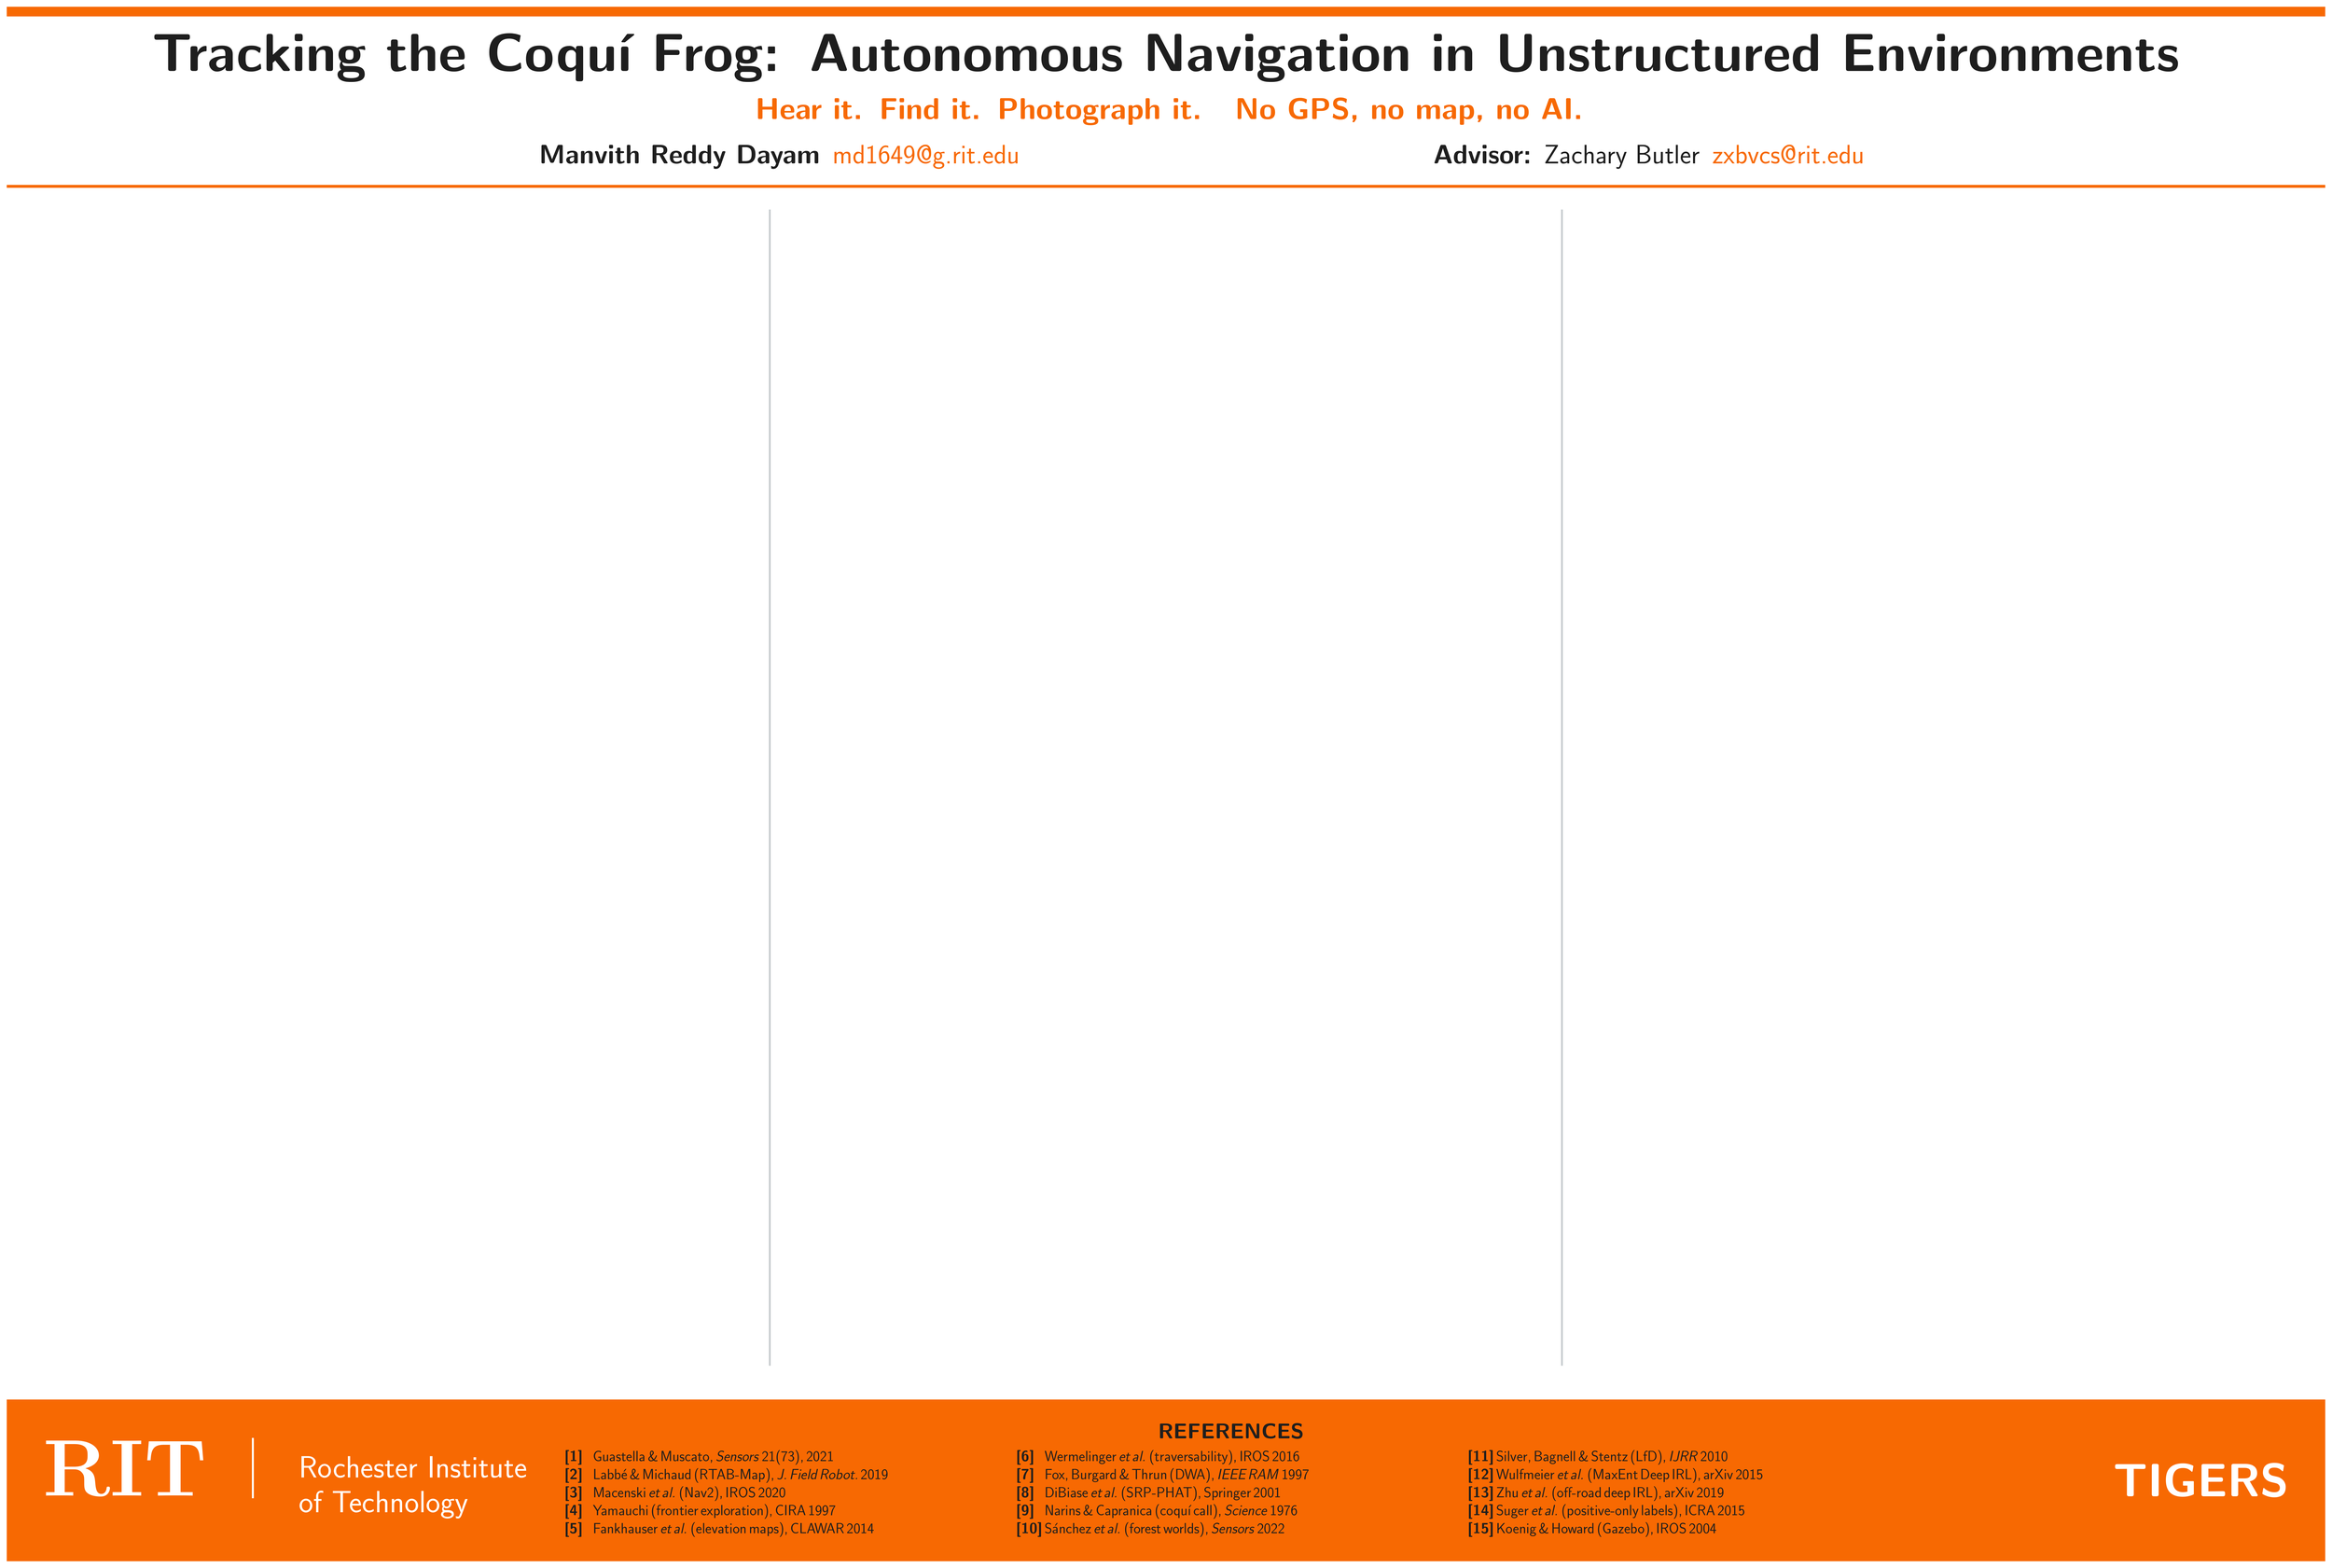
\begin{tikzpicture}[x=1in,y=1in]
  \useasboundingbox (0,0) rectangle (48,32.2);
  % ---- title band (white, orange rules) ----
  \fill[ritorange] (0,32.0) rectangle (48,32.2);
  \fill[ritorange] (0,28.45) rectangle (48,28.51);
  \node[text width=46in, align=center, font=\titlesize\bfseries, text=ritdark]
       at (24,31.12) {\strut\PosterTitle};
  \node[text width=46in, align=center, font=\taglinesize\bfseries, text=ritorange]
       at (24,30.02) {\strut\PosterTagline};
  \node[anchor=base, font=\authorsize, text=ritdark] at (16,28.95)
       {\textbf{\AuthorName}\enspace\textcolor{ritorange}{\AuthorEmail}};
  \node[anchor=base, font=\authorsize, text=ritdark] at (34,28.95)
       {\textbf{Advisor:}\enspace\AdvisorName\enspace\textcolor{ritorange}{\AdvisorEmail}};
  % ---- column separators ----
  \draw[ritgray!45, line width=2.5pt] (0.75+14.6+0.45,4.05) -- ++(0,23.95);
  \draw[ritgray!45, line width=2.5pt] (0.75+14.6+0.9+15.5+0.45,4.05) -- ++(0,23.95);
  % ---- footer band ----
  \fill[ritorange] (0,0) rectangle (48,3.35);
  \node[anchor=west, inner sep=0pt] at (0.75,1.675) {%
    \IfFileExists{\FigRITLogo}{\includegraphics[height=1.4in]{\FigRITLogo}}{%
      \color{white}\fontsize{120}{120}\selectfont\rmfamily\bfseries RIT\enspace
      \rule[-0.05in]{3pt}{1.25in}\enspace
      \sffamily\mdseries\fontsize{46}{52}\selectfont
      \begin{tabular}[c]{@{}l@{}}Rochester Institute\\ of Technology\end{tabular}}};
  \node[anchor=east, inner sep=0pt] at (47.25,1.675) {%
    \IfFileExists{\FigRITSign}{\includegraphics[height=2.75in]{\FigRITSign}}{%
      \color{white}\fontsize{70}{70}\selectfont\bfseries\itshape TIGERS}};
  \node[text width=27.6in, align=center, text=ritdark] at (25.35,1.675) {%
    {\fontsize{32}{38}\selectfont\bfseries REFERENCES\par}\vspace{0.1in}
    \refsize\raggedright
    \begin{minipage}[t]{8.9in}
      \rf{1}Guastella \& Muscato, \textit{Sensors}~21(73), 2021\\
      \rf{2}Labb\'e \& Michaud (RTAB-Map), \textit{J.\,Field Robot.}~2019\\
      \rf{3}Macenski \textit{et al.} (Nav2), IROS~2020\\
      \rf{4}Yamauchi (frontier exploration), CIRA~1997\\
      \rf{5}Fankhauser \textit{et al.} (elevation maps), CLAWAR~2014
    \end{minipage}\hfill
    \begin{minipage}[t]{8.9in}
      \rf{6}Wermelinger \textit{et al.} (traversability), IROS~2016\\
      \rf{7}Fox, Burgard \& Thrun (DWA), \textit{IEEE RAM}~1997\\
      \rf{8}DiBiase \textit{et al.} (SRP-PHAT), Springer~2001\\
      \rf{9}Narins \& Capranica (coqu\'i call), \textit{Science}~1976\\
      \rf{10}S\'anchez \textit{et al.} (forest worlds), \textit{Sensors}~2022
    \end{minipage}\hfill
    \begin{minipage}[t]{8.9in}
      \rf{11}Silver, Bagnell \& Stentz (LfD), \textit{IJRR}~2010\\
      \rf{12}Wulfmeier \textit{et al.} (MaxEnt Deep IRL), arXiv~2015\\
      \rf{13}Zhu \textit{et al.} (off-road deep IRL), arXiv~2019\\
      \rf{14}Suger \textit{et al.} (positive-only labels), ICRA~2015\\
      \rf{15}Koenig \& Howard (Gazebo), IROS~2004
    \end{minipage}\par};
\end{tikzpicture}}}

% =====================================================================
\begin{document}
\noindent
% =====================================================================
%  COLUMN 1 -- question, the frog, why it is hard, previous work, goal
% =====================================================================
\begin{minipage}[t][\colH][t]{\colA}
\bodysize

\sect{\faQuestionCircle}{Research Question}
\begin{keybox}
\fontsize{34}{43}\selectfont
Can \textbf{pure math} -- geometry, filtering and graph search -- drive a robot
through \textbf{unstructured terrain} \emph{without AI} or learning from
demonstration?
\end{keybox}

\sectgap
\sect{\faFrog}{Our Test: Find This Frog}
\begin{minipage}[c]{6.1in}
  The \textbf{coqu\'i} is about 5\,cm long and hides in grass, bushes and trees.
  But it shouts its own name all night: \emph{``co''} warns rivals,
  \emph{``qu\'i''} calls mates~[9].\par
  \vspace{0.12in}
  {\fontsize{31}{38}\selectfont\bfseries\color{ritorange}Can't see it? Listen.\par}
\end{minipage}\hfill
\begin{minipage}[c]{8.2in}
  \slot[0.4]{\FigCall}{\linewidth}{Spectrogram of the call}
\end{minipage}\par

\sectgap
\sect{\faMountain}{Why Off-Road Is Hard}
\begin{tikzpicture}[x=1in,y=1in]
  \card{0}{1.92}{\faTree}{Every tree looks alike.}{Place recognition gets fooled.}
  \card{7.4}{1.92}{\faSeedling}{Grass looks like a wall.}{LiDAR can't tell soft from solid.}
  \card{0}{0}{\faMountain}{The ground isn't flat.}{2D maps break on slopes.}
  \card{7.4}{0}{\faCog}{Wheels slip.}{Six wheels scrub on every turn.}
\end{tikzpicture}

\sectgap
\sect{\faBook}{Previous Work}
\begin{itemize}[leftmargin=1.9em, labelsep=0.5em, itemsep=0.42em]
  \item[\ico{\faMap}] \textbf{Map it.} Graph SLAM builds the map and finds the
        robot in it~[2]; frontiers say where to look next~[4].
  \item[\ico{\faRoute}] \textbf{Cross it.} Elevation maps score steps and
        slopes~[5,6]; Nav2 plans a path and DWA drives it~[3,7].
  \item[\ico{\faBrain}] \textbf{Learn it.} Learning from demonstration copies an
        expert's feel for good ground~[1,11--13].
  \item[\ico{\faTimes}] \textbf{The catch:} experts only show where they
        \emph{did} drive, so the robot never sees a bad example~[14].
\end{itemize}

\sectgap
\begin{goalbox}
\fontsize{31}{39}\selectfont
\textcolor{ritteal}{\bfseries\faBullseye\enspace OUR GOAL}\par\vspace{0.06in}
Build \textbf{wild, realistic} worlds, push pure math until it \textbf{breaks},
and see which link snaps first:
\textcolor{ritorange}{\bfseries Sense}, \textcolor{ritorange}{\bfseries Plan} or
\textcolor{ritorange}{\bfseries Act}.
\end{goalbox}
\end{minipage}%
\hspace{\colgap}%
% =====================================================================
%  COLUMN 2 -- experimental setup
% =====================================================================
\begin{minipage}[t][\colH][t]{\colB}
\bodysize

\sect{\faCogs}{Experimental Setup}
\subhead{One rover, three jobs
  {\mdseries\color{inkgray}\enspace(ROS\,2, Nav2~[3], Gazebo~[15])}}
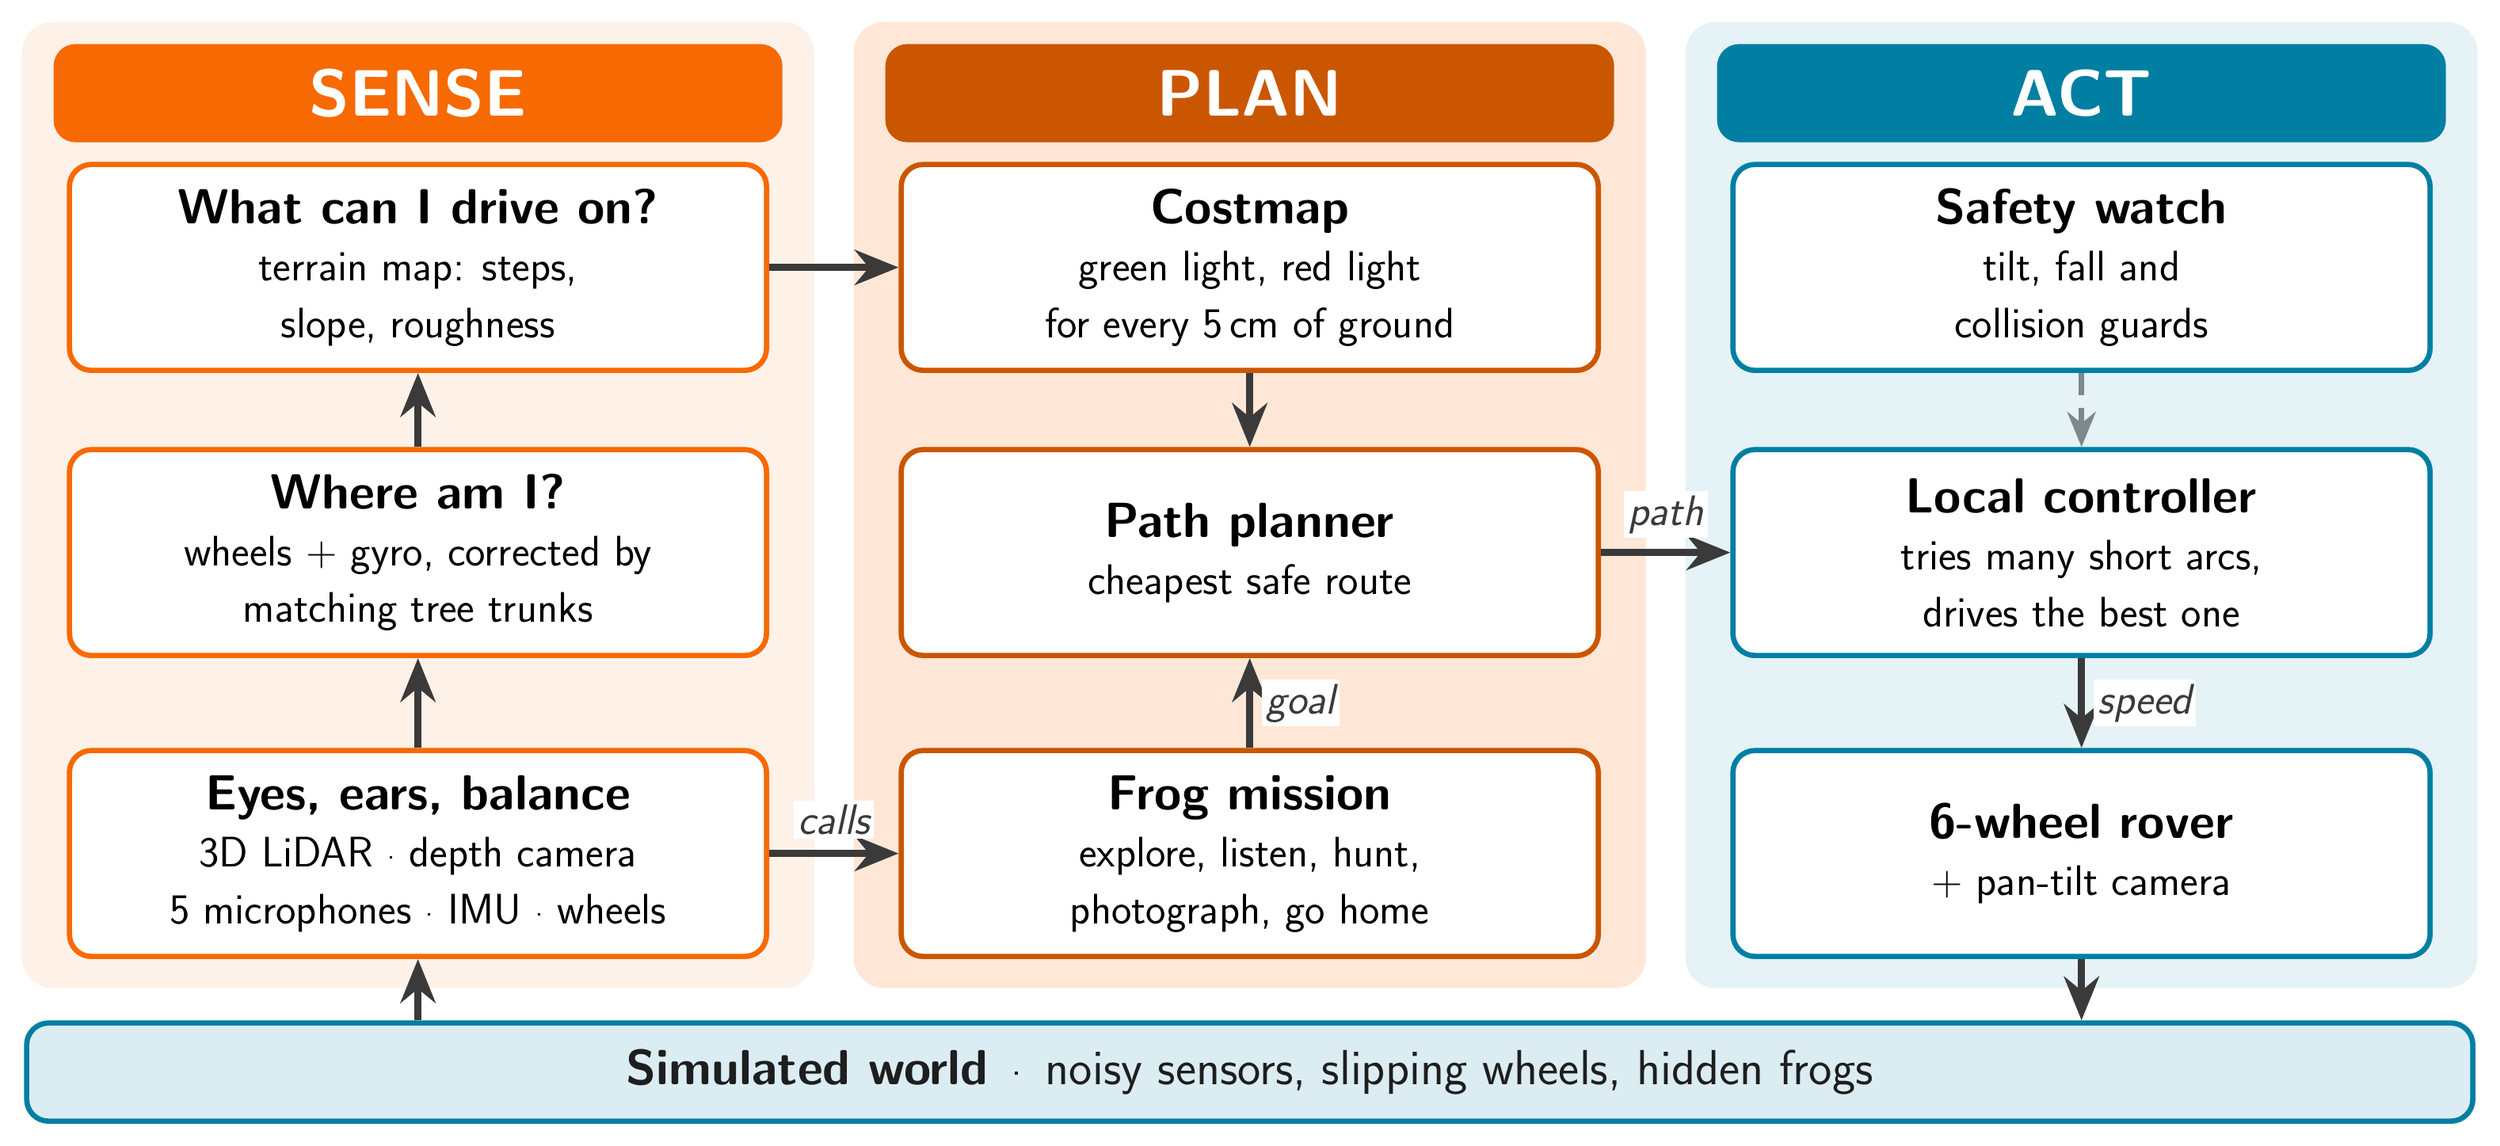
\begin{tikzpicture}[x=1in,y=1in]
  % lanes (exactly 15.5in wide)
  \fill[lane=ritorange!9]  (0,0.85)     rectangle (5.0,6.95);
  \fill[lane=ritorange!16] (5.25,0.85)  rectangle (10.25,6.95);
  \fill[lane=ritteal!10]   (10.5,0.85)  rectangle (15.5,6.95);
  \node[lanehead=ritorange]          at (2.5,6.5)   {SENSE};
  \node[lanehead=ritorange!82!black] at (7.75,6.5)  {PLAN};
  \node[lanehead=ritteal]            at (13.0,6.5)  {ACT};
  % SENSE (bottom -> top)
  \node[blk=ritorange] (s1) at (2.5,1.7)
    {\textbf{Eyes, ears, balance}\\{\diagsmall 3D LiDAR \textperiodcentered{} depth camera}\\{\diagsmall 5 microphones \textperiodcentered{} IMU \textperiodcentered{} wheels}};
  \node[blk=ritorange] (s2) at (2.5,3.6)
    {\textbf{Where am I?}\\{\diagsmall wheels + gyro, corrected by}\\{\diagsmall matching tree trunks}};
  \node[blk=ritorange] (s3) at (2.5,5.4)
    {\textbf{What can I drive on?}\\{\diagsmall terrain map: steps,}\\{\diagsmall slope, roughness}};
  % PLAN
  \node[blk=ritorange!82!black] (p3) at (7.75,5.4)
    {\textbf{Costmap}\\{\diagsmall green light, red light}\\{\diagsmall for every 5\,cm of ground}};
  \node[blk=ritorange!82!black] (p2) at (7.75,3.6)
    {\textbf{Path planner}\\{\diagsmall cheapest safe route}};
  \node[blk=ritorange!82!black] (p1) at (7.75,1.7)
    {\textbf{Frog mission}\\{\diagsmall explore, listen, hunt,}\\{\diagsmall photograph, go home}};
  % ACT
  \node[blk=ritteal] (a3) at (13.0,5.4)
    {\textbf{Safety watch}\\{\diagsmall tilt, fall and}\\{\diagsmall collision guards}};
  \node[blk=ritteal] (a2) at (13.0,3.6)
    {\textbf{Local controller}\\{\diagsmall tries many short arcs,}\\{\diagsmall drives the best one}};
  \node[blk=ritteal] (a1) at (13.0,1.7)
    {\textbf{6-wheel rover}\\{\diagsmall + pan-tilt camera}};
  % world bar
  \node[draw=ritteal, line width=2.4pt, fill=ritteal!14, text=ritdark, rounded corners=10pt,
        minimum width=15.44in, minimum height=0.62in, inner sep=0pt, font=\diagsize] (gz) at (7.75,0.32)
    {\textbf{Simulated world}\enspace\textperiodcentered\enspace noisy sensors, slipping wheels, hidden frogs};
  % flows
  \draw[flow] (gz.north -| s1) -- (s1);
  \draw[flow] (s1) -- (s2);
  \draw[flow] (s2) -- (s3);
  \draw[flow] (s3) -- (p3);
  \draw[flow] (p3) -- (p2);
  \draw[flow] (p1) -- node[lab, right=4pt]{goal} (p2);
  \draw[flow] (s1) -- node[lab, above=5pt]{calls} (p1);
  \draw[flow] (p2) -- node[lab, above=5pt]{path} (a2);
  \draw[feed] (a3) -- (a2);
  \draw[flow] (a2) -- node[lab, right=4pt]{speed} (a1);
  \draw[flow] (a1) -- (gz.north -| a1);
\end{tikzpicture}

\subgap
\subhead{Four worlds, from easy to brutal}
\begin{tikzpicture}[x=1in,y=1in]
  \world{0}{\faLeaf}{Park}{warm-up lap}
  \world{3.925}{\faWater}{Lake}{slippery shore}
  \world{7.85}{\faTree}{Forest}{look-alike trees}
  \world{11.775}{\faMountain}{Hill}{steep climbs}
\end{tikzpicture}

\subgap
\begin{minipage}[t]{0.488\linewidth}\centering
  \slot{\FigWorldA}{\linewidth}{Gazebo forest world}
  \figcap{\textbf{(a)}~The forest \dots}
\end{minipage}\hfill
\begin{minipage}[t]{0.488\linewidth}\centering
  \slot{\FigWorldB}{\linewidth}{LiDAR map}
  \figcap{\textbf{(b)}~\dots{} and what the robot's LiDAR makes of it}
\end{minipage}

\subgap
% frog_tree.jpg is from an earlier mission (fast_final); the others are from the two
% forest missions reported in Results.
\subhead{Caught on camera
  {\mdseries\color{inkgray}\enspace(taken by the robot, three missions)}}
\begin{minipage}[t]{0.238\linewidth}\centering
  \slot{\FigFrogA}{\linewidth}{Frog in the open}
  \figcap{in the open}
\end{minipage}\hfill
\begin{minipage}[t]{0.238\linewidth}\centering
  \slot{\FigFrogB}{\linewidth}{Frog in a bush}
  \figcap{inside a bush}
\end{minipage}\hfill
\begin{minipage}[t]{0.238\linewidth}\centering
  \slot{\FigFrogC}{\linewidth}{Frog up a tree}
  \figcap{up a tree}
\end{minipage}\hfill
\begin{minipage}[t]{0.238\linewidth}\centering
  \slot{\FigFrogD}{\linewidth}{Frog in tall grass}
  \figcap{heard, never seen}
\end{minipage}

\sectgap
\begin{warnbox}{When the simulator lies}
The forest~[10] was built for a bigger robot. Its trail edges were \textbf{4--9\,cm
cliffs} to our 4\,cm wheels, and 268 tufts of grass were \textbf{solid as rock}:
the rover flipped. We fixed the world, not the robot.
Test drives passed: \textbf{8 of 24} $\to$
\textcolor{ritorange}{\textbf{24 of 24}}.
\end{warnbox}
\end{minipage}%
\hspace{\colgap}%
% =====================================================================
%  COLUMN 3 -- audio tracking, results, learnings, conclusion
% =====================================================================
\begin{minipage}[t][\colH][t]{\colC}
\bodysize

\sect{\faMicrophone}{Audio \& Call Tracking}
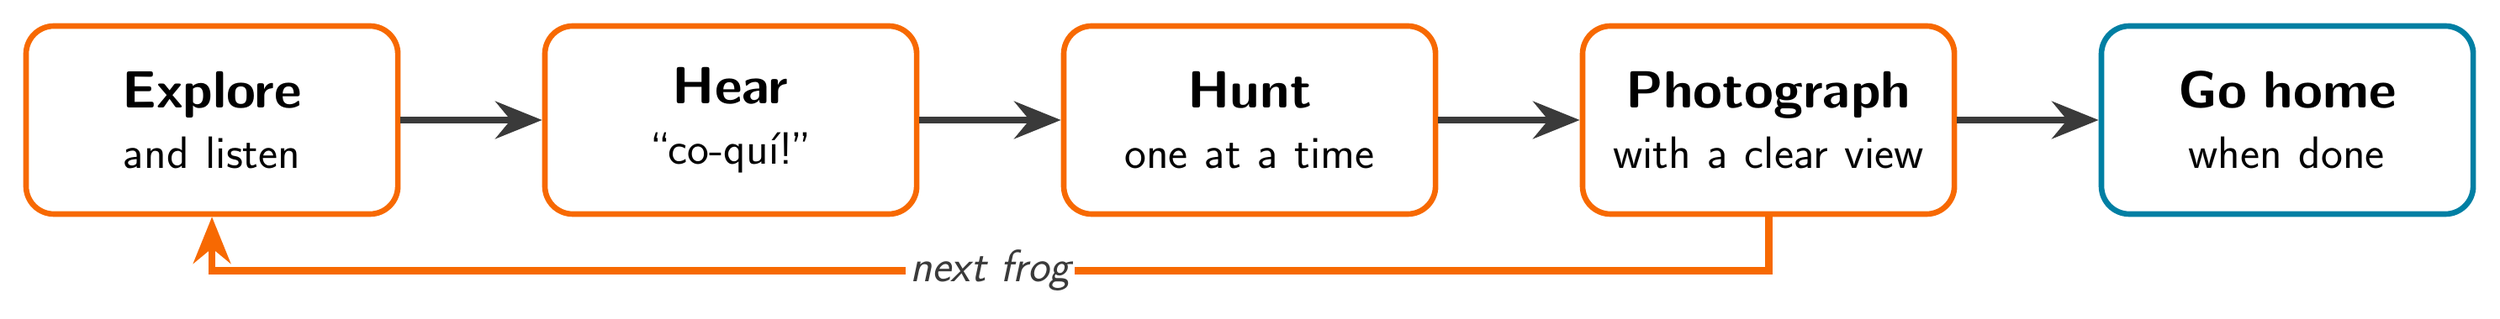
\begin{tikzpicture}[x=1in,y=1in]
  \node[state] (e) at (1.13,0)  {\textbf{Explore}\\{\diagsmall and listen}};
  \node[state] (h) at (4.215,0) {\textbf{Hear}\\{\diagsmall ``co-qu\'i!''}};
  \node[state] (v) at (7.3,0)   {\textbf{Hunt}\\{\diagsmall one at a time}};
  \node[state] (c) at (10.385,0){\textbf{Photograph}\\{\diagsmall with a clear view}};
  \node[state, draw=ritteal] (r) at (13.47,0) {\textbf{Go home}\\{\diagsmall when done}};
  \foreach \a/\b in {e/h,h/v,v/c,c/r} \draw[flow] (\a) -- (\b);
  \draw[flow, draw=ritorange] (c.south) -- ++(0,-0.32) -| node[lab, pos=0.25]
       {next frog} (e.south);
\end{tikzpicture}

\vspace{0.14in}
% ---- triangulation, as a picture instead of equations ----
\begin{tikzpicture}[x=1in,y=1in]
  \useasboundingbox (0,0) rectangle (14.6,3.25);
  \coordinate (frog) at (4.3,2.72);
  \draw[ritgray, line width=3pt, dash pattern=on 12pt off 9pt]
       (0.2,0.62) .. controls (1.6,0.35) and (2.9,0.5) .. (4.1,0.62)
                  .. controls (5.4,0.75) and (6.4,0.5) .. (8.4,0.62);
  \draw[ritorange, line width=5pt] (1.0,0.55) -- (frog);
  \draw[ritorange, line width=5pt] (4.1,0.6)  -- (frog);
  \draw[ritorange, line width=5pt] (7.2,0.6)  -- (frog);
  \draw[ritgray, line width=3.5pt, dash pattern=on 10pt off 8pt] (7.2,0.6) -- (8.75,2.45);
  \node[roverstop] at (1.0,0.55) {\faRobot};
  \node[roverstop] at (4.1,0.6)  {\faRobot};
  \node[roverstop] at (7.2,0.6)  {\faRobot};
  \node[circle, fill=white, inner sep=3pt, text=ritteal,
        font=\fontsize{66}{66}\selectfont] at (frog) {\faFrog};
  \node[circle, fill=white, inner sep=3pt, text=ritgray,
        font=\fontsize{46}{46}\selectfont] at (8.75,2.45) {\faFrog};
  \node[anchor=east, font=\diagsize\bfseries, text=ritteal] at (3.5,2.85) {it must be here};
  \node[anchor=south, font=\diagsmall\itshape, text=inkgray, inner sep=1pt] at (8.75,2.93) {not this one};
  \node[anchor=west, align=left, text width=4.85in, inner sep=0pt] at (9.75,1.62)
    {\fontsize{25.5}{31}\selectfont
     \ico{\faMicrophone}\enspace 5 mics: a \textbf{direction}~[8]\par\vspace{0.1in}
     \ico{\faRoute}\enspace 3 stops: a \textbf{distance}\par\vspace{0.1in}
     \ico{\faVolumeUp}\enspace loudness: \textbf{which frog}\par};
\end{tikzpicture}

\sectgap
\sect{\faChartLine}{Results: Did It Work?}
% Forest: runs claude_full1 (designed layout) and claude_rand3 (random layout, seed 3), 6/6 each,
% 0 false, mean horizontal error 0.14 m and 0.20 m (0.17 m over the 12 frogs).
% Hill: run claude_hill1, 3/6, 0 false, ended by hand after 10 min below a bank it could not climb.
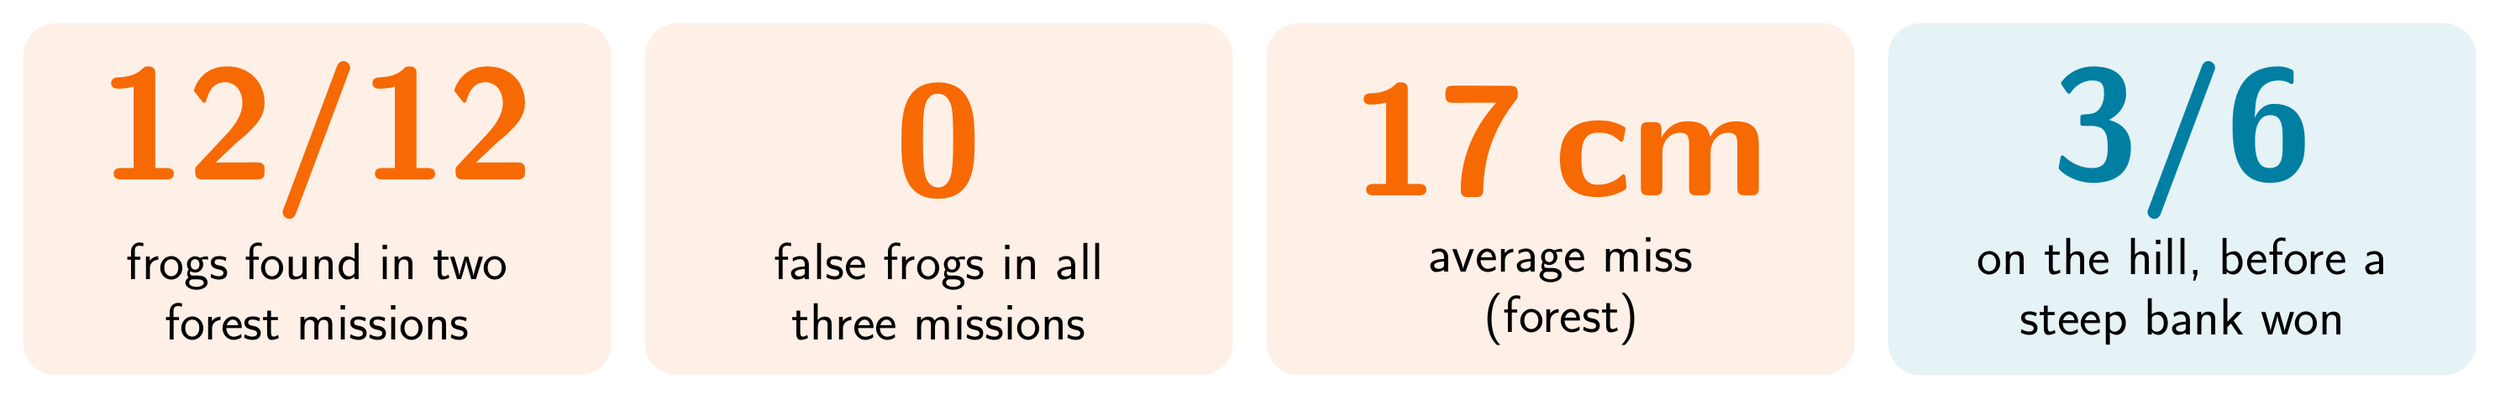
\begin{tikzpicture}[x=1in,y=1in]
  \tile{0}{12/12}{frogs found in two\\forest missions}{ritorange}
  \tile{3.7}{0}{false frogs in all\\three missions}{ritorange}
  \tile{7.4}{17\,cm}{average miss\\(forest)}{ritorange}
  \tile{11.1}{3/6}{on the hill, before a\\steep bank won}{ritteal}
\end{tikzpicture}

\vspace{0.16in}
\begin{minipage}[t]{8.0in}\centering
  \slot[0.66875]{\FigMap}{\linewidth}{Mission map}
  \figcap{\textbf{(c)}~One simulated mission: 330\,m, 19\,min, 6 of 6 frogs}
\end{minipage}\hfill
\begin{minipage}[t]{6.4in}\centering
  \slot[0.8359375]{\FigDrift}{\linewidth}{Position error}
  \figcap{\textbf{(d)}~Same drive, three ways to stay found}
\end{minipage}

\sectgap
\sect{\faLightbulb}{Key Learnings}
\begin{enumerate}[label={\badge{\arabic*}}, leftmargin=1.75em, labelsep=0.45em,
                  itemsep=0.32em]
  \item \textbf{The world isn't flat.} 3D odometry plus tree matching cut the
        worst error from 4.7\,m to 0.4\,m.
  \item \textbf{Follow one voice.} Mixing two callers invented frogs that were
        never there.
  \item \textbf{Geometry can't feel.} Grass it could push through still looks
        like a wall.
\end{enumerate}

\sectgap
\sect{\faFlagCheckered}{Conclusion}
\textbf{In the forest, yes; on the steep hill, not yet.} Plain math found every
forest frog. What broke was mostly \textcolor{ritorange}{\textbf{Sense}}, not the
planner. Next: keep the math and \textbf{learn only the terrain cost}~[11--13].
\end{minipage}

\end{document}
